\section{Relative pose estimation}
\label{sec:relative_pose}

\subsection{Iterative Closest learned-Point}
\begin{algorithm}
 \KwData{initial pose $\mathbf{h}_{init}$, point cloud to align $\mathcal{P}$ with associated descriptors $\mathcal{D}$ and reference point cloud $\mathcal{P}_{ref}$ with assocaited descriptors $\mathcal{D}_{ref}$}
 \KwResult{final pose $\mathbf{h}_{refined}$}
% initialization\;
 $\mathbf{h}_{refined} \gets \mathbf{h}_{init}$\;
 $\mathbf{h}_{relative} \gets \mathbf{1}_{4\times 4}$\;
 \While{$\norm{\mathbf{h}_{relative} - \mathbf{I}_{4\times 4}}_{\mathrm{F}} \geq \epsilon $}{
    $\mathcal{P}_{aligned} \gets \mathbf{h}_{refined}\mathcal{P}$\;
	$\mathcal{M} \gets \mathtt{match\_points}(\mathcal{P}_{aligned}, \mathcal{P}_{ref}, \mathcal{D}, \mathcal{D}_{ref})$\;  
	$\mathbf{h}_{relative} \gets \mathtt{relative\_pose}(\mathcal{M})$\;
    $\mathbf{h}_{refined} \gets \mathbf{h}_{relative}\mathbf{h}_{refined}$\;
 }
 \If{$\norm{\mathcal{M}}_2 > \epsilon_{repro}$}{
     $\mathbf{h}_{refined} \gets \mathbf{h}_{init}$\;
 }

 \caption{\label{alg:icp}Our ICP algorithm, see text for details about functions $\mathtt{match\_points}$ and $\mathtt{relative\_pose}$. Pose refinement is rejected if the mean distance between matched points, $\norm{\mathcal{M}}_2$, is superior to $\epsilon_{repro}$.}
\end{algorithm}
\label{subsec:pc_alignment}
Thanks to the dense geometric information provided the encoder-decoder network, we can rely on robust ICP algorithm to refine the initial pose. 

\paragraph{Local point cloud.}
With the generated depth map obtained by our neural network and the intrinsic parameters of the camera, we can project the depth map on the point cloud $\mathcal{P}_{I}$:
\begin{equation}
	\left[\mathcal{P}_{I}\right]_{l + k\times W_d} = \mathbf{p}_{l + k\times W_d} = \left[\mathbf{F}^{\mathrm{D}}_I\right]_{k,l} \cdot \mathbf{K}^{-1}[k, l, 1]^T,
\end{equation}
where $\mathbf{p}\in\mathbb{R}^{3}$ is a 3D point and $\left[\cdot\right]_j$ is the subscription operator at index $j$. $\mathcal{P}_{I}$ contains $W_d \times H_d$ 3D points.

\paragraph{Point descriptor.}
Refinement with ICP involves matching corresponding points between two point clouds in order to estimate a rigid transformation that minimises the distances between the paired points. Standard approaches only consider the Euclidean distance between a single point and its nearest neighbours in the reference point cloud to establish matching, making the initial alignment between the two point clouds a crucial step to obtain correct results. We can rely on point descriptors to establish strongest matches~\cite{Pomerleau2015}. Because the point cloud to align is generated with a deep neural network, we associate to each projected point $\mathbf{p}$ a $C$-dimensional descriptor $\mathbf{d}\in\mathbb{R}^{C}$ corresponding to the deep feature computed by the encoder $\mathrm{E}$ at the same spatial position:
\begin{equation}
	\left[ \mathcal{D}_{I} \right]_{l + k\times W_d} =  \mathbf{d}_{l + k\times W_d} = \left[ \mathbf{G}^{\mathrm{E}}_{I} \right]_{k, l},
\end{equation}
where $\mathcal{D}_{I}$ is set set of point descriptors associated to point cloud $\mathcal{P}_{I}$ and $\mathbf{G}^{\mathrm{E}}_{I} \in\mathbb{R}^{C\times H_d\times W_d}$ are the feature maps from $\mathrm{E}$ that have the same spatial resolution that the output of $\mathrm{D}$.

\noindent Descriptors $\mathcal{D}$ are obtained without any additional computation cost because latent features $\mathbf{G}^{\mathrm{E}}_{I}$ have already been computed by $\mathrm{E}$ to produce final features $\mathbf{F}^{\mathrm{E}}_{I}$.

\paragraph{Global point cloud.} 
To align the point cloud generated from the query, we need a reference scene geometry. We sample a pool of reference data within a fixed radius centred on the initial retrieved pose $\mathbf{h}_{\mathrm{i}}$. The reference point cloud $\mathcal{P}_{ref}$ is created by aggregating all the point clouds from these data (using ground truth or generated depth maps). We also compute point descriptors $\mathcal{D}_{ref}$ corresponding to the 3D points in $\mathcal{P}_{ref}$.
\noindent The reference point cloud is computed offline and stored efficiently for fast access during query time.

\paragraph{Pose refinement.}
Final refined pose $\mathbf{h}_{\mathrm{r}}$ is given by:
\begin{equation}
	\mathbf{h}_{\mathrm{r}} = \mathtt{ICP}(\mathbf{h}_{\mathrm{i}}, \mathcal{P}_{I_q}, \mathcal{D}_{I_q}, \mathcal{P}_{ref}, \mathcal{D}_{ref}),
\end{equation}
where $\mathtt{ICP}$ is the function described in algorithm~\ref{alg:icp}. The $\mathtt{match\_points}$ function computes pairs of similar points both based on the spatial proximity and on the descriptors similarity. In other words, two pairs of point descriptors $\left\{ \mathbf{p}_m, \mathbf{d}_m \right\}$ and $\left\{ \mathbf{p}_n, \mathbf{d}_n\right\}$ are matched together if:
\begin{equation}
m, n = \underset{k, l}{\mathrm{argmin}} \norm{\left[\mathbf{p}_k, \mathbf{d}_k \right] - \left[\mathbf{p}_l, \mathbf{d}_l\right]}_2,
\end{equation}
where $\left[\cdot\right]$ is the concatenation operator. The matches are retrieved efficiently by $k$-d tree fast nearest neighbour search. The $\mathtt{relative\_pose}$ function computes the relative transformation between the matched points that minimises the Euclidean difference between the two point clouds. We embed the pose computation within a \ac{ransac}, as the point cloud may contain erroneous data because it has been generated from image-only information by our encoder/decoder.

\subsection{Perspective-n-learned-Points}
\begin{figure}
	\centering
	
    \begin{minipage}{0.5\linewidth}
    		\subfigure[][PnlP]{\label{fig:pnlp}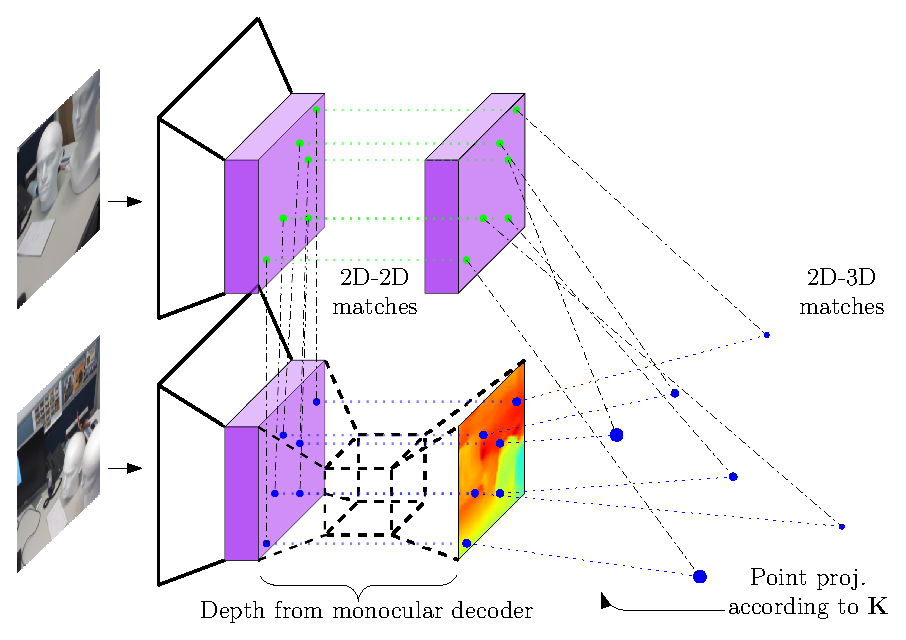
\includegraphics[width=0.9\linewidth]{method/pnlp.eps}}
    \end{minipage}\hfill
	\begin{minipage}{0.5\linewidth}
   		\subfigure[][IClP]{\label{fig:iclp}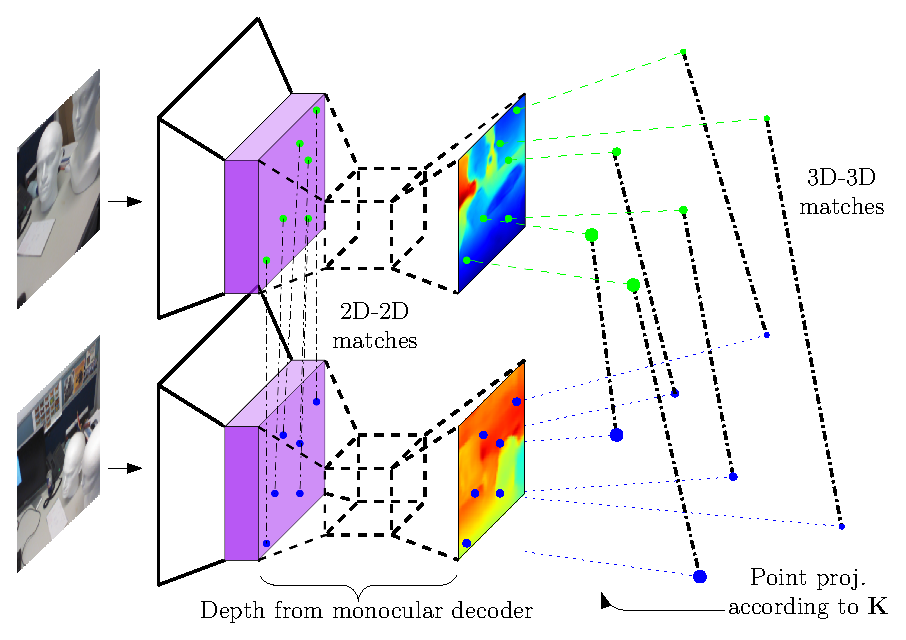
\includegraphics[width=0.9\linewidth]{method/iclp.eps}}
	\end{minipage}
	
	\caption[]{\textbf{:} \ref{fig:pnlp} \ref{fig:iclp} \label{fig:relative_pose}}
\end{figure}

\label{subsec:pnlp}
Thanks to the generated depth map (section~\ref{subsec:depth_map}) and the equation~\ref{eq:3d_proj}, we can project 2D points from retrieved images into 3D coordinates. 2D-2D correspondences obtained in section~\ref{subsec:matching} can be interpreted as 2D-3D correspondences and we can use PnP algorithm to compute the relative transformation $\mathbf{h}_\mathrm{r \rightarrow q}$ between the query image and the reference image. 

We embed the PnP algorithm within a RANSAC consensus where a sub-part of 2D-3D correspondences are evaluated at a time. As we have multiple reference candidates from image retrieval step (section~\ref{subsec:image_indexing}), we select the pose with the largest proportion of inlier correspondences after the PnP optimisation. If the ratio of inlier is below a given threshold, we simply affect the pose of the retrieved image to the query.

\subsection{Final pose computation}
We obtain final pose of query image $\mathrm{I_q}$ using the relation:
\begin{equation}
	\mathbf{h}_\mathrm{q} = \mathbf{h}_\mathrm{r}\mathbf{h}_\mathrm{r \rightarrow q}.
\end{equation}

\subsection{System design and motivation}
\paragraph{Multi-task model.} In order to make our system fast and lightweight, we use a single encoder/decoder neural network for the three tasks needed in our pose estimation pipeline. That means with a single image forward, we obtain a compact global image description, dense local descriptors and a depth map corresponding to the observed scene.
\paragraph{Single task training policy.} There are dedicated training pipeline for each of the computer vision tasks involved in our image pose estimation framework: methods for learning a global image descriptor~\citep{Arandjelovic2017, Radenovic2017, Gordo2017}, CNN designed to extract and describe local features~\citep{Yi2016a, Rocco2018, Ono2018} and system that produces a depth map from a monocular image~\citep{Eigen2014, Godard2017, Mahjourian2018}. We decide to train our encoder/decoder network for the task of depth from monocular estimation because estimation of erroneous depth measurement will result in wrong estimation of the final pose. In the next section, we experimentally show that even if our network has not been trained especially for the task of image description or local feature matching, the latent features computed within the network embed enough high-level semantic to perform well on these tasks~\citep{Taira2018, Zamir2018}.
\paragraph{Generalisation.} Because we rely on a non-absolute representation of the scene geometry (depth is estimated \textit{relatively} to the camera frame), our model is not limited to localisation on one specific scene like end-to-end pose estimation networks~\citep{Kendall2017, Brachmann2017b}. In other words, the same trained network can be used to localise images in multiple indoor and outdoor scenes, and even on totally unknown environments. 
%Our model can also benefit from dense scene geometry when available during training or relying only on weakly annotated data
